\section{Descrizione generale}
\subsection{Contesto d'utilizzo}
%review the contents of this section
Il \glossaryItem{progetto} \glossaryItem{MaaS} mira a fornire un servizio online per le aziende per la visualizzazione dei propri dati aziendali attraverso un'interfaccia grafica. In particolare il \glossaryItem{progetto} intende creare un ambiente di sviluppo online per la modellazione di queste interfacce, in modo semplice e veloce per gli sviluppatori.
Tale scopo è parzialmente raggiunto dall'applicazione \glossaryItem{MaaP}, la quale è un \glossaryItem{framework} che offre gli strumenti necessari agli sviluppatori per creare tali interfacce. Quest'applicativo tuttavia richiede l'installazione del framework necessario in un server per l'azienda che ne vuole usufruire, operazione onerosa che richiede conoscenze informatiche molto spesso assenti nelle aziende. \glossaryItem{MaaS} cerca di colmare questa lacuna tramite un servizio: una piattaforma raggiungibile online che non necessita dei passaggi di installazione per l'utente, ma solo di un passaggio di registrazione per creare un proprio spazio.

\subsection{Funzione di Prodotto}
%review the contents of this section
\glossaryItem{MaaS} dovrà fornire all'utente una piattaforma su cui effettuare la registrazione per la propria \glossaryItem{Company}. Effettuato questo passaggio, un \glossaryItem{Owner} pu\`o invitare i propri collaboratori al servizio ed aggiungere gli accessi al proprio database \glossaryItem{MongoDB} per poter creare le viste.
Oltre a questo, \glossaryItem{MaaS} punta ad estendere le funzionalità di \glossaryItem{MaaP} tramite un editor per la creazione delle viste, strumento in grado di agevolare l'utente nella gestione delle proprie interfacce.


\subsection{Entit\`a}
Le entit\`a (e le relazioni esistenti tra di loro) definite nel modello \glossaryItem{SaaS} di \glossaryItem{MaaS} vengono esposte di seguito. La loro descrizione \`e stata utile nell'identificazione delle varie tipologie di attori per la trattazione dei casi d'uso.
\begin{description}
	\item[\glossaryItem{Company}] \hfill \\\\
	Una \glossaryItem{Company} \`e un'entit\`a in relazione con gli utenti: un insieme di utenti appartiene a una \glossaryItem{Company} e ciascun utente deve appartenere a una \glossaryItem{Company};
	\item[Utente] \hfill \\\\
	Ogni utente appartenente ad una \glossaryItem{Company} ha un ruolo; a ciascun ruolo sono associate diverse funzioni.	
	
	I ruoli sono i seguenti: \glossaryItem{Owner}, \glossaryItem{Admin}, \glossaryItem{Member}, \glossaryItem{Guest}.	
	Ciascuna funzione associata ad un ruolo pu\`o essere eseguita solo nell'ambito della \glossaryItem{Company} di appartenenza. \\\\
	\textbf{Ruoli e funzioni} \hfill \\\\
		Il seguente elenco dei ruoli rispecchia la gerarchia individuata per gli attori nei casi d'uso.
                 \begin{figure}[H]
                   \begin{center}
                     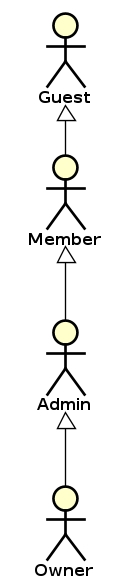
\includegraphics[width=0.15\textwidth]{res/img/UCUtenti/gerarchia_utenti.png}
                     \caption{Gerarchia degli utenti}
                   \end{center} 
                 \end{figure}  
		\begin{description}
			\item[\glossaryItem{Guest}] Pu\`o eseguire il \glossaryItem{DSL} a cui ha accesso.
			\item[\glossaryItem{Member}] Pu\`o eseguire, leggere e scrivere una specifica \glossaryItem{DSL} a cui ha accesso e crearne una nuova.
			\item[\glossaryItem{Admin}] Pu\`o eseguire qualsiasi operazione sul \glossaryItem{DSL} appartenente alla relativa \glossaryItem{Company}. Pu\`o invitare altri utenti, aggiungere/togliere/modificare ruoli e aggiungere/togliere/modificare permessi in lettura/scrittura al \glossaryItem{DSL}.
			\item[\glossaryItem{Owner}] Pu\`o eseguire le stesse funzioni dell'\glossaryItem{Admin}, non pu\`o essere eliminato e pu\`o impersonare altri utenti all-interno della \glossaryItem{Company}
                         %%%%%ancora problemi di formattazione?
                        \item[\glossaryItem{Super-Admin}] \hfill \\\\
	Il \glossaryItem{Super-Admin} non appartiene a nessuna \glossaryItem{Company}. Questo ruolo \`e utile per gli amministratori di sistema, che hanno il compito di fornire supporto agli utenti.
		\end{description}
\end{description}

\subsection{Vincoli \textit{software} generali}

\newpage
